So far a number of algorithms for control, trajectory optimization, motion planning, perception, and localization/state estimation have been presented. Almost all of these instances share a common characteristic: they involve manipulation or observation of \textit{continuous} variables. For example, motion planning and control algorithms manipulate the robot's physical state (i.e. position, velocity, orientation, configuration) which can take on a continuous range of values, and perception and localization tasks try to take (continuously valued) information from the environment and try to estimate the robot's physical state. 

However, for higher-level tasks it is often useful to represent the state of the robot or environment in terms of a discrete set of variables. For example, consider a robot whose task is to go from point A to point B, pick up a package, and then deliver it to point C. While the robot's physical (continuous) state is crucial for tasks such as controlling the robot to drive from A to B, it is also important to keep track of what portion of the overall plan that the robot is currently performing (is the robot currently traversing to B or C, has the package been successfully picked up, etc.). Additionally, it might be useful to keep track of other discrete valued states of the robot, such as if a sensor is functioning or not, or whether or not the robot is in the presence of a human (i.e. for safety).
Similar to dynamics/kinematics models for the robot's (continuous) physical state, \textit{finite state machines}\cite{KaelblingWhiteEtAl2011} are a useful framework for modeling discrete higher-level states of the robot and its environment.

\notessection{Finite State Machines}
Finite state machines (FSMs) define a computational modeling framework for systems whose output depends on the entire history of their inputs, and where the number of possible states of the system is \textit{finite}. This framework has been used in a wide variety of disciplines, including electrical engineering, linguistics, computer science, philosophy, biology, and more. FSMs can also be used in several different ways, including:
\begin{enumerate}
    \item {\em to specify a desired program or behavior}, such as how a vending machine or ATM should function,
    \item {\em to model behavior}, for example to analyze the behavior of a control system interacting with the environment,
    \item {\em or for predicting behavior}, for example to predict what will happen in the future given some set of inputs to the system.
\end{enumerate}

Generally speaking, designing finite state machines for practical robotic systems can be extremely time consuming and challenging. In particular, choosing the appropriate set of states for a particular problem is required to ensure that the model is not overly complex, but the interactions and transitions between states can also be very hard to specify and can still lead to complex models. For example, consider the graphical representation of an example FSM for the popular open source flight software PX4 in Figure \ref{fig:px4fsm}. Specifying the full behavior of the system can lead to a complex FSM, even if there are not very many states. In fact, this FSM is still under continuous development to improve the overall system behavior!
\begin{figure}[ht]
    \centering
    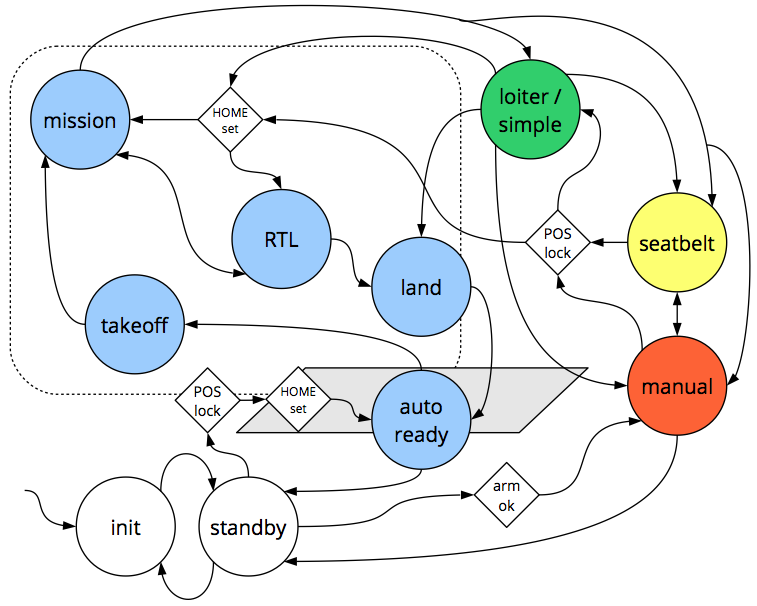
\includegraphics[width=0.65\textwidth]{tex/figs/ch21_figs/px4_state_machine.png}
    \caption{A graphical representation of a finite state machine example for the open source flight software PX4, \texttt{https://px4.io/}. As can be seen, even for a relatively small number of states the FSM can become quite complex in order to model the full behavior of the system. Image retrieved from diydrones.com.}
    \label{fig:px4fsm}
\end{figure}

Mathematically, a finite state machine consists of:
\begin{enumerate}
    \item a \textit{finite} set of states $S$,
    \item a set of inputs $I$,
    \item a set of outputs $O$,
    \item a next-state function $n(i_t, s_t) \xrightarrow{} s_{t+1}$ that maps the input $i_t$ at time $t$ and current state $s_t$ to the next state $s_{t+1}$,
    \item an output function $o(i_t, s_t) \xrightarrow{} o_t$,
    \item and an initial state $s_0$.
\end{enumerate}
While FSMs can be defined through the mathematical notation above, it is often also useful to represent them graphically to get a more intuitive understanding of how the system will behave. In particular, the graph representation is defined with nodes of the graph representing each state in the set $S$. Each (directed) edge of the graph corresponds to a possible transition between states that is defined by a particular input. In other words, each directed edge is associated with a particular pair $(s, i)$. The outputs for a particular pair $(s,i)$ are also typically included along each directed edge. This is shown in more detail in Figure \ref{fig:fsm}.
\begin{figure}[ht]
    \centering
    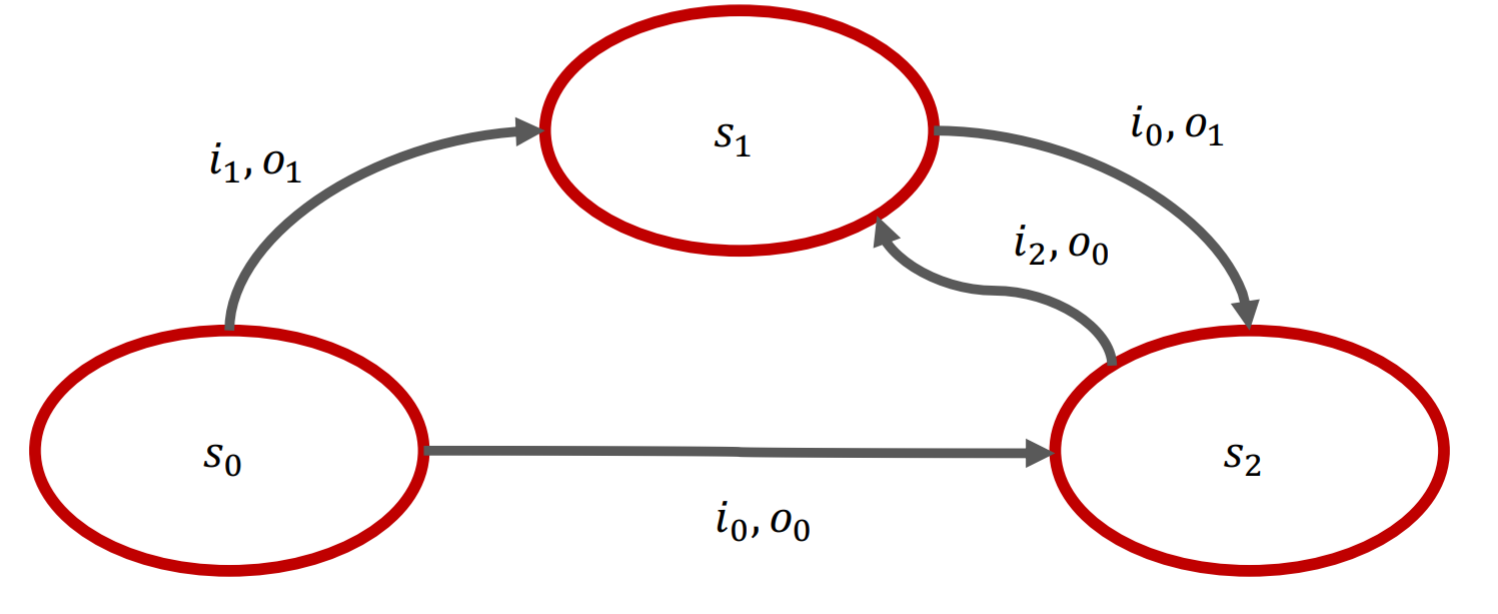
\includegraphics[width=0.65\textwidth]{tex/figs/ch21_figs/fsm.png}
    \caption{A graphical representation of a finite state machine with states $S = \{s_0, s_1, s_2\}$, inputs $I = \{i_0,i_1,i_2\}$ and outputs $O = \{o_0, o_1\}$. The directed edges correspond to the next-state functions and the output associated with each edge is defined by the output function. For example, in this FSM it can be seen that $n(i_1, s_0) \xrightarrow{} s_1$ and $o(i_1, s_0) \xrightarrow{} o_1$.}
    \label{fig:fsm}
\end{figure}

\begin{example}[Parking Gate Control] \label{ex:parkinggate}
\theoremstyle{definition}
Consider a parking gate control finite state machine where the goal is to raise the gate when a car arrives and then lower the gate when the car has passed. Assume sensors are available to tell if a car is at the gate and when the car has passed through the gate, and also the position of the gate. The control actions the gate can take are simply raising, lowering, or holding the gate position fixed. Technically, the position of the gate can vary continuously between the ``down'' and ``up'' positions, and the velocity can also vary continuously. However, in designing a finite state machine to define the overall logic/behavior for the parking gate, a higher-level abstraction of the set of gate states can be chosen as:
\begin{equation*}
S = \{\text{down}, \: \text{raising}, \:\text{up},\: \text{lowering}\}.
\end{equation*}
The set of inputs to the finite state machine come from the sensors, and can be chosen as:
\begin{equation*}
\begin{split}
I = \{&\text{car waiting}, \: \text{no car waiting}, \:\text{car passed},\: \text{car not passed},\: \\ &\text{gate up}, \: \text{gate not up},\: \text{gate down},\: \text{gate not down} \}.    
\end{split}
\end{equation*}
Finally, the output of the finite state machine (defining the actions for the gate) are simply:
\begin{equation*}
O = \{\text{lower}, \: \text{raise}, \:\text{hold}\}.
\end{equation*}

The next-state function then defines the desired behavior for the parking gate. For example, suppose the current state $s_t = \text{down}$ and the sensor measures that a car is waiting ($i_t = \text{car waiting}$). Then, the desired behavior is to output the command $o_t = \text{raise}$, and the next-state function would be:
\begin{equation*}
    n(\text{car waiting}, \text{down}) \xrightarrow{} \text{raising}.
\end{equation*}
Similarly, suppose the gate was just raised for the car to pass such that $s_t = \text{up}$, but that the sensor is giving input $i_t = \text{car not passed}$. In this case the output would be $o_t = \text{hold}$, and the next-state function would be:
\begin{equation*}
    n(\text{up}, \text{car not passed}) \xrightarrow{} \text{up}.
\end{equation*}
A graphical representation of the full car parking gate FSM is given in Figure \ref{fig:parkinggate}.
\begin{figure}[ht]
    \centering
    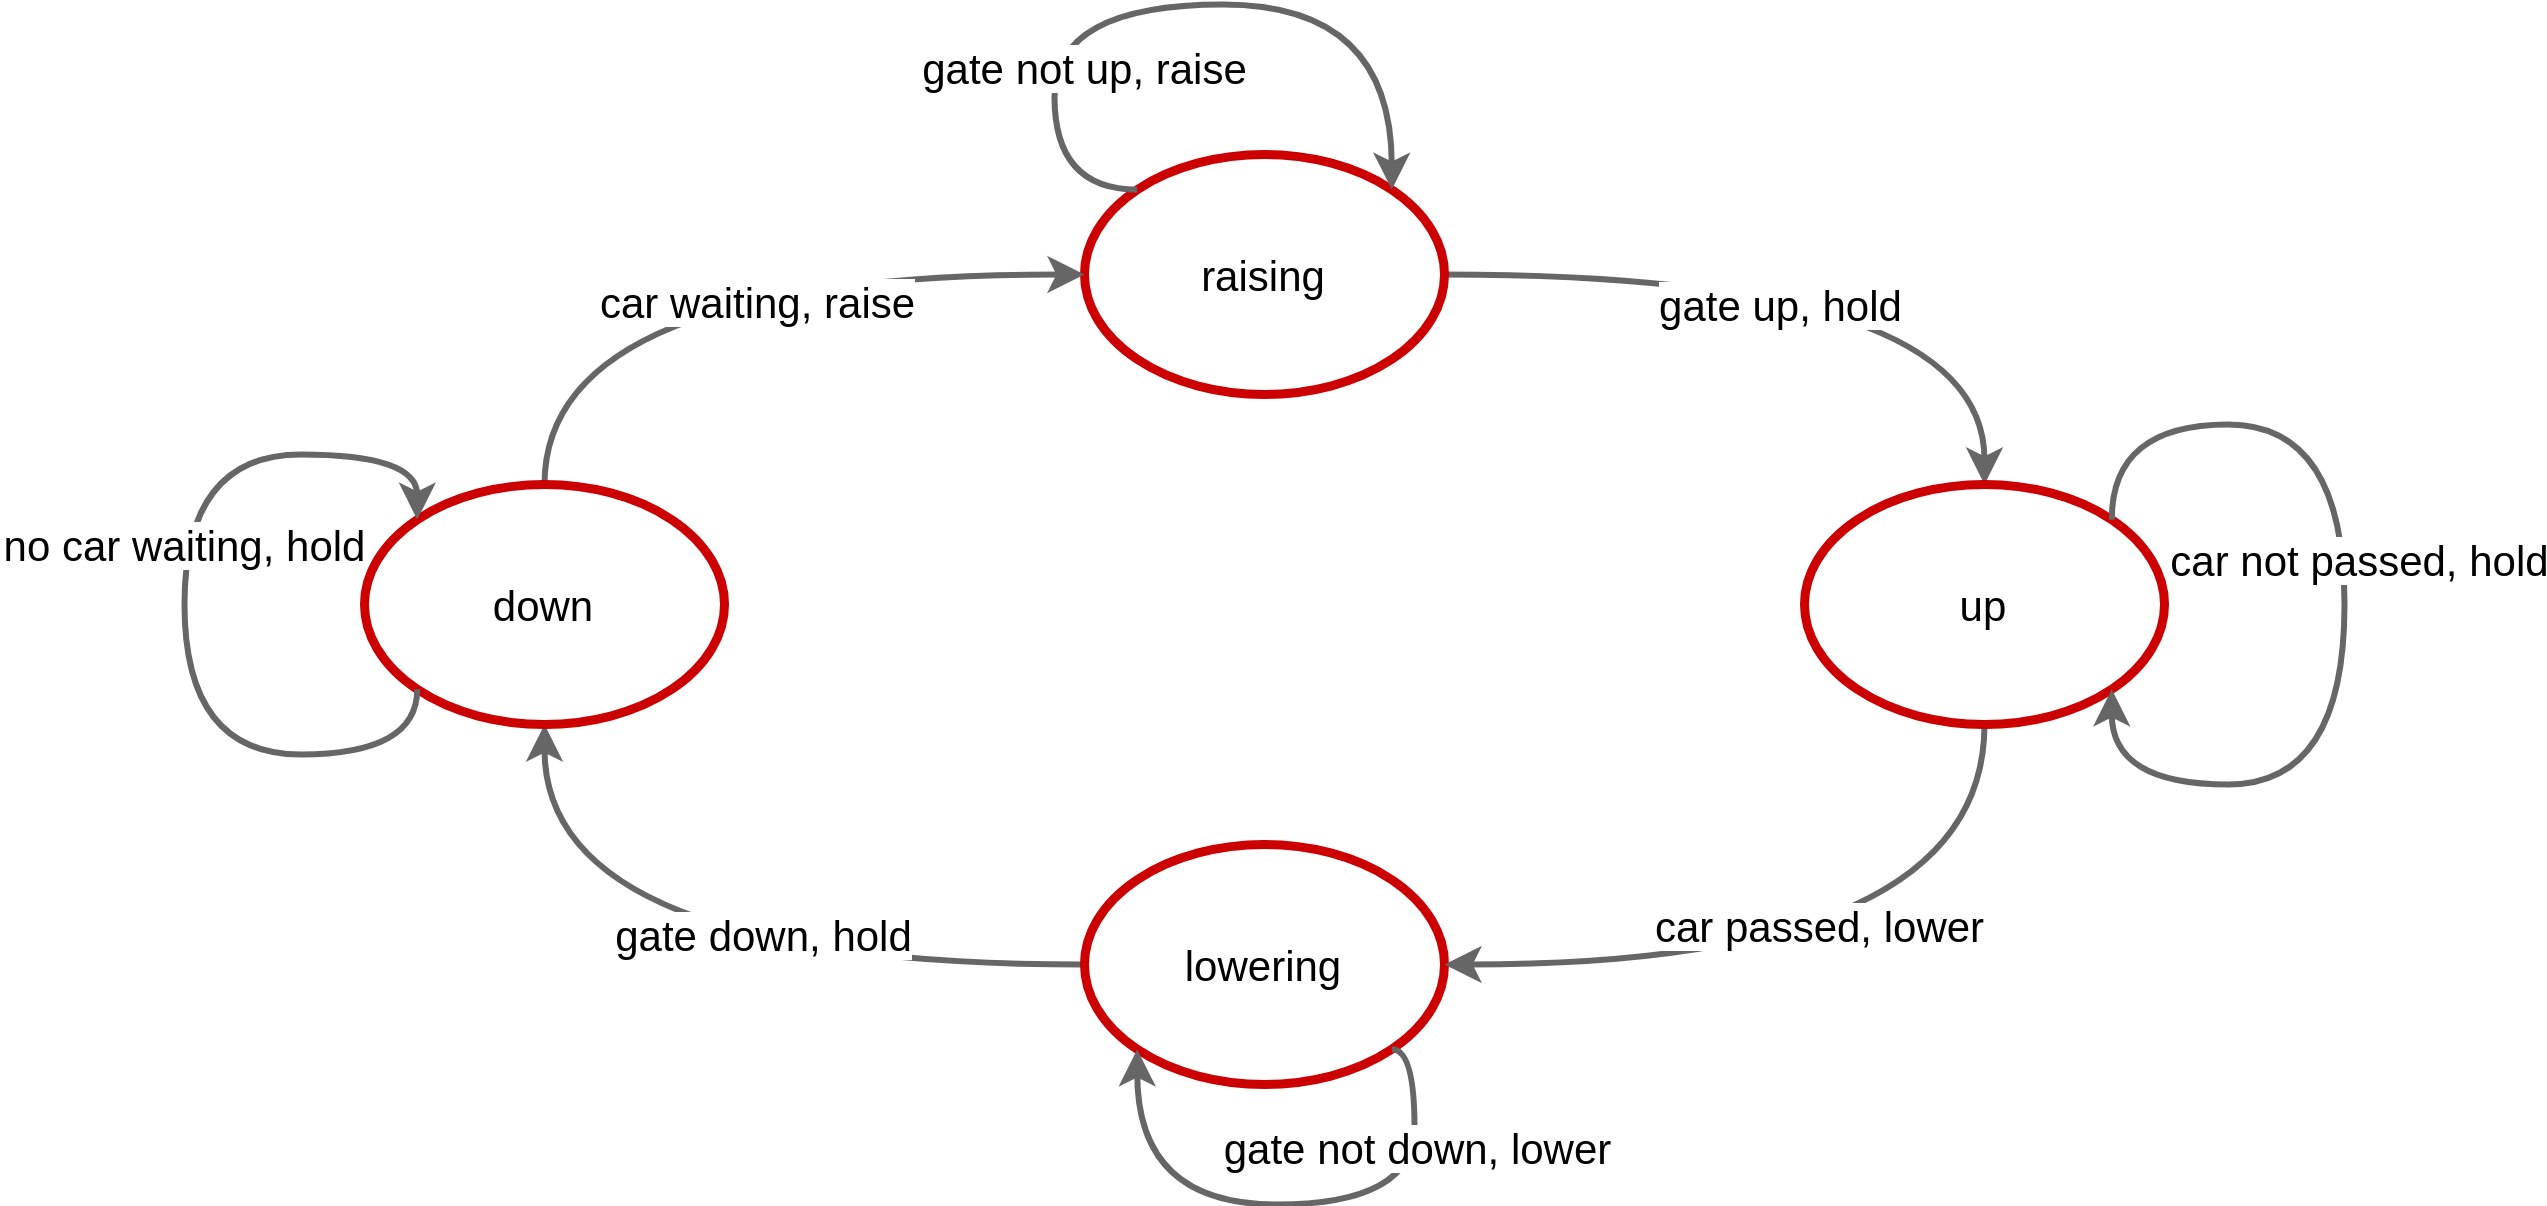
\includegraphics[width=1\textwidth]{tex/figs/ch21_figs/parkinggate_fsm.png}
    \caption{A graphical representation of the finite state machine for the parking gate controller discussed in Example \ref{ex:parkinggate}.}
    \label{fig:parkinggate}
\end{figure}
\end{example}

\subsection{FSM Architectures}
Finite state machines can become quite complex since for every new state added it is possible to define an exponentially increasing number of new transitions. Strategies for keeping the complexity of FSMs in check include analyzing for (and removing) redundant states, using hierarchical FSMs, and using compositions based on common patterns.

\subsubsection{Reducing Number of States}
There exist algorithms that can be used to identify and combine states in FSMs that would yield the same overall behavior. In particular, two states are equivalent if they have the same output and for all input combinations transition to the same or equivalent states.

One possible algorithm for reducing states in an FSM is as follows:
\begin{enumerate}
    \item Place all states into one set.
    \item Create a single partition based on the output behavior.
    \item Repeatedly partition further based on next state transitions until no further partitions is possible.
\end{enumerate}
To see this procedure in action, consider the following example:
\begin{example}[FSM State Reduction] \label{ex:sequence}
\theoremstyle{definition}
Consider a finite state machine that is used to detect the sequences 010 or 110. The FSM is shown in Table \ref{tab:sequence}, where it can be seen that the states are the partial sequences $S = \{0,1,00,01,10,11\}$ and a reset state, the inputs are $I = \{0,1\}$, and the outputs are booleans $O = \{\text{True}, \text{False} \}$ for whether the sequence 010 or 110 has been created. For example, it can be seen that if the current partial sequence is 01 ($s_4$) and a 0 is input, the next state will be the reset state and the output will be True.
\begin{table}[ht]
\centering
\begin{tabular}{|l|
>{\columncolor[HTML]{C0C0C0}}l |l|
>{\columncolor[HTML]{C0C0C0}}l |l|}
\hline
State, $s$ & $n(0,s)$ & $n(1,s)$ & $o(0,s)$ & $o(1,s)$ \\ \hline
Reset      & 0        & 1        & False    & False    \\ \hline
0          & 00       & 01       & False    & False    \\ \hline
1          & 10       & 11       & False    & False    \\ \hline
00         & Reset    & Reset    & False    & False    \\ \hline
01         & Reset    & Reset    & True     & False    \\ \hline
10         & Reset    & Reset    & False    & False    \\ \hline
11         & Reset    & Reset    & True     & False    \\ \hline
\end{tabular}
\caption{Finite state machine for a sequence detector that accepts digits 0 and 1 and outputs True if the sequences 010 or 110 is generated.}
\label{tab:sequence}
\end{table}

Now, the FSM in Table \ref{tab:sequence} can be simplified by removing redundant states! This is accomplished by first placing all of the states into a single set $\{\text{Reset}, 0, 1, 00, 01, 10, 11\}$ and creating a partition based on the output behavior. In particular this will generate two sets:
\begin{equation*}
\begin{split}
\{\text{Reset}, 0, 1, 00, 10\}&: \text{always leads to False output},\\
\{01,11\}&: \text{does not always lead to False output}.
\end{split}
\end{equation*}
These sets are then further partitioned based on the next-state function until no further partitions can be made. In the first step the set $\{\text{Reset}, 0, 1, 00, 10\}$ is partitioned into:
\begin{equation*}
\begin{split}
\{\text{Reset}, 00, 10\}&: \text{cannot transition to \{01,11\}},\\
\{0, 1\} &: \text{can transition to \{01,11\}}.
\end{split}
\end{equation*}
and then $\{\text{Reset}, 00, 10\}$ is partitioned as:
\begin{equation*}
\begin{split}
\{\text{Reset}\}&: \text{can transition to \{0, 1\}},\\
\{00, 10\}&: \text{cannot transition to \{0, 1\}}.
\end{split}
\end{equation*}
Therefore, instead of the original seven states (Reset, $0$, $1$, $00$, $01$, $10$, $11$) there are now only four ($\{01,11\}$, $\{0, 1\}$, Reset, $\{00, 10\}$).
An equivalent (same input/output behavior) but reduced finite state machine can now be defined, and is shown in Table \ref{tab:sequence2}.
\begin{table}[ht]
\centering
\begin{tabular}{|l|
>{\columncolor[HTML]{C0C0C0}}l |l|
>{\columncolor[HTML]{C0C0C0}}l |l|}
\hline
State, $s$                        & $n(0,s)$  & $n(1,s)$                          & $o(0,s)$ & $o(1,s)$ \\ \hline
Reset                             & \{0,1\}   & \{0,1\}                           & False    & False    \\ \hline
\{0,1\}                           & \{00,10\} & \cellcolor[HTML]{FFFFFF}\{01,11\} & False    & False    \\ \hline
\cellcolor[HTML]{FFFFFF}\{00,10\} & Reset     & Reset                             & False    & False    \\ \hline
\cellcolor[HTML]{FFFFFF}\{01,11\} & Reset     & Reset                             & True     & False    \\ \hline
\end{tabular}
\caption{Reduced finite state machine for a sequence detector that accepts digits 0 and 1 and outputs True if the sequences 010 or 110 is generated.}
\label{tab:sequence2}
\end{table}

\subsubsection{Hierarchical FSMs}
In some cases there might be states that are not truly equivalent, but that might still be beneficial to group closely together. With this idea, the concepts of \textit{super-states} (i.e. groups of closely related states) and \textit{generalized transitions} (i.e. transitions between super-states) can be useful. This idea of creating super-states is analogous to graph clustering.

\subsubsection{Compositions}
Individual state machines can also be composed in a variety of ways depending on their input/output behavior, including \textit{cascade} compositions, \textit{parallel} compositions, and \textit{feedback} compositions. Cascade compositions combine two FSMs in sequence where the output vocabulary of one matches the input vocabulary of the other. The new state of the combined machine is the concatenation of the states of the individual FSMs (see Figure \ref{fig:cascade}). Parallel compositions run two FSMs side by side, using the same input. Both the state and output is then the concatenation of the two individual FSMs' state and output. Finally, feedback compositions use only a single FSM but only require a partial input and also reuse the output as input (requires the input and output vocabularies to be the same). \begin{marginfigure}
    \centering
    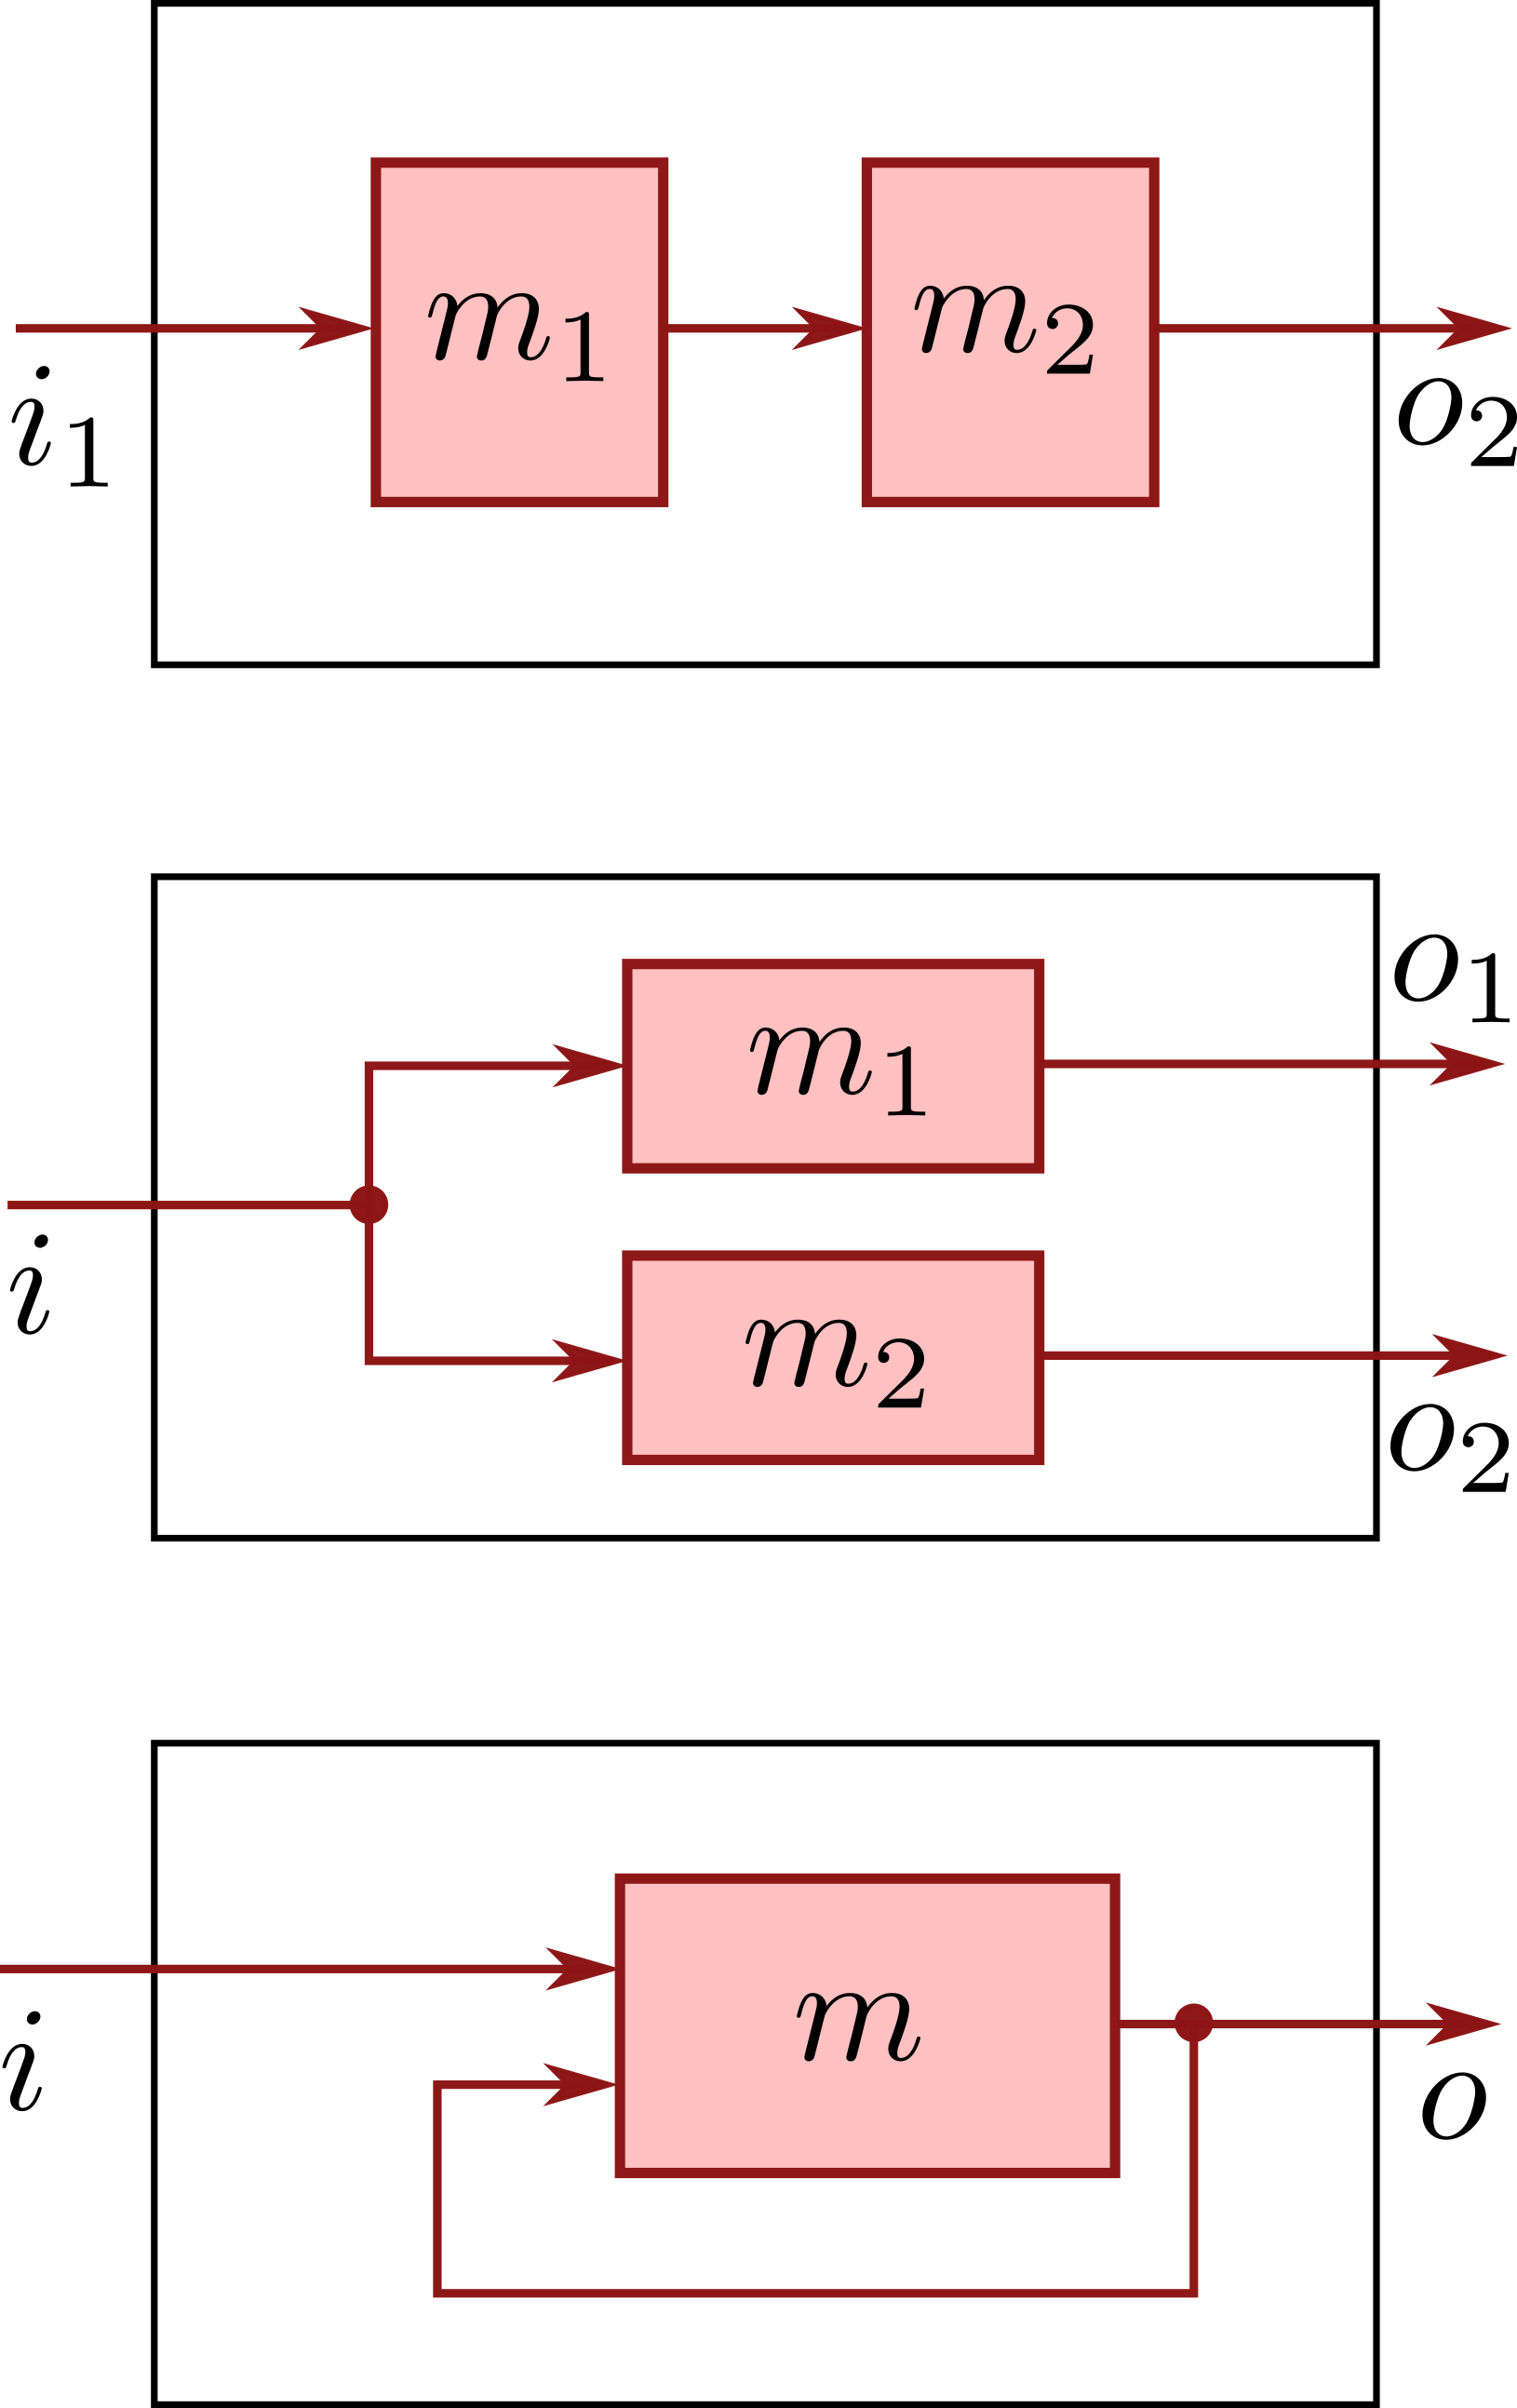
\includegraphics[width=0.8\textwidth]{tex/figs/ch21_figs/compositions.png}
    \caption{Cascade, parallel, and feedback compositions of finite state machines.}
    \label{fig:cascade}
\end{marginfigure}



\subsection{Implementation Details}
There are \textit{numerous} ways that finite state machines could be implemented in practice. However, one common approach is to exploit Object Oriented Programming (OOP) by building the finite state machine as a class. In particular, the class would keep track of the state of the FSM in a class variable. The state update process could then occur through the use of if/else statements in an update class method, as well as the definition of the FSM output. An example implementation in Python of the parking gate controller FSM from Example \ref{ex:parkinggate} is given below:
\begin{python}
import rospy as rp
from std_msgs.msg import String

class ParkingGateFSM():
    """Simple FSM for parking gate control"""
    def __init__(self):
        rp.init_node('parking_gate', anonymous=True)
        self.state = 'down'
        self.cmd = rp.Publisher('/gate_cmd', String)
        rp.Subscriber('/car_sensor', String, self.car_clbk)
        rp.Subscriber('/gate_sensor', String, self.gate_clbk)

    def car_clbk(self, data):
        self.car_input = data

    def gate_clbk(self, data):
        self.gate_input = data

    def run(self):
        rate = rp.Rate(10) # 10 Hz
        while not rp.is_shutdown():
            if self.state == 'down':
                if self.car_input == 'no_car_waiting':
                    output = 'hold'
                elif self.car_input == 'car_waiting':
                    self.state = 'raising'
                    output = 'raise'
            elif self.state == 'raising':
                if self.gate_input == 'gate_not_up':
                    output = 'raise'
                elif self.gate_input == 'gate_up':
                    self.state = 'up'
                    output = 'hold'
            elif self.state == 'up':
                if self.car_input == 'car_not_passed':
                    output = 'hold'
                elif self.car_input == 'car_passed':
                    self.state = 'lowering'
                    output = 'lower'
            elif self.state == 'lowering':
                if self.gate_input == 'gate_not_down':
                    output = 'lower'
                elif self.gate_input == 'gate_down':
                    self.state = 'down'
                    output = 'hold'
            self.cmd.publish(output)
            rate.sleep()
\end{python}

\subsection{Other Useful Tools}
A useful tool for visualizing finite state machines in ROS is SMACH, which can be though of as an analogue to RViz. More information about SMACH and how it is used can be found on the ROS Wiki\footnote{http://wiki.ros.org/smach}. 
\end{example}